\documentclass[tikz,border=11pt]{standalone}
\usetikzlibrary{arrows.meta, positioning, calc, math}

\def\rthick{0.2} % rectangle thickness

\tikzset{
  poststyle/.style={thick, fill=blue!20},
  compstyle/.style={thick, fill=green!20},
  sendstyle/.style={thick, fill=red!20},
  recvstyle/.style={thick, fill=orange!20}
}

% rankcontroller arg#1: height of the timeline box
\newcommand{\rankcontroller}[1]{%
  % place a coordinate rx at (2, 0)
  \coordinate (ctl) at (2, 0);
  \coordinate (agg) at (8, 0);
  \coordinate (mpi) at (14, 0);

  \begin{scope}[shift={(-0.0, 0)}]
    \draw[->,thick,-stealth] (0, 0) -- (0, -#1);
  \end{scope}

  \begin{scope}[shift={(ctl)}]
    \node[rankbox] (ry) at (0,0) {$Controller$};
    \draw[style=dotted] (ry.south) -- (0, -#1);
  \end{scope}

  \begin{scope}[shift={(agg)}]
    \node[rankbox] (ry) at (0,0) {$Aggregator$};
    \draw[style=dotted] (ry.south) -- (0, -#1);
  \end{scope}

  \begin{scope}[shift={(mpi)}]
    \node[rankbox] (rx) at (0,0) {$Rank\ 0$};
    \draw[style=dotted] (rx.south) -- (0, -#1);
  \end{scope}
}

\begin{document}
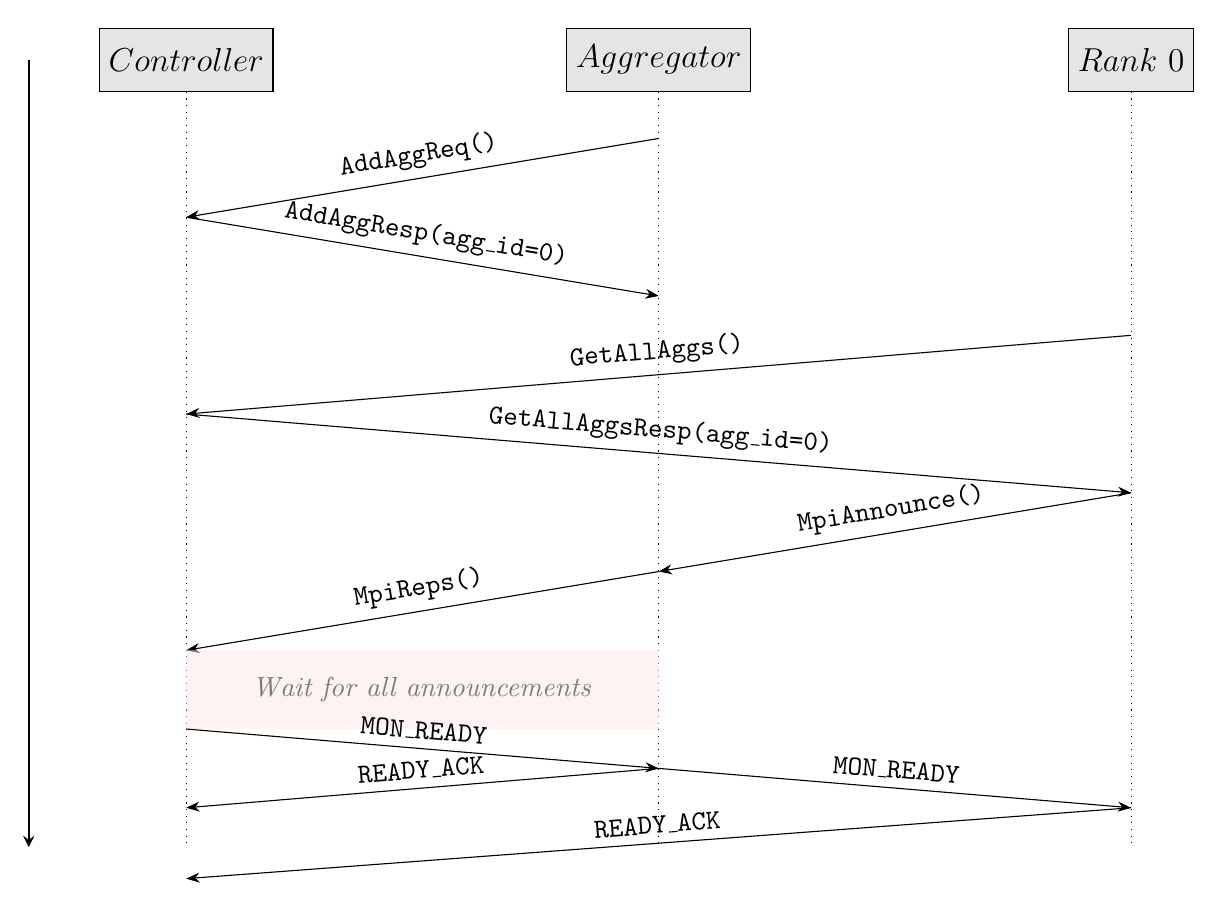
\begin{tikzpicture}[
    rankbox/.style={rectangle, draw, minimum width=1.5cm, minimum height=0.8cm, fill=gray!20, font=\large},
    thread/.style={dotted, thick},
    seqnode/.style={font=\ttfamily\normalsize},
    arrow/.style={->,-Stealth},
    font=\normalsize
  ] % temporary, to visualize grid
  % \draw[step=1cm, gray!10, very thin] (-4, -10) grid (10, 4);
    \rankcontroller{10}

    \draw[arrow] ([yshift=-1cm] agg) -- ([yshift=-2cm] ctl)
        node[midway, above, sloped, seqnode]{AddAggReq()};
    \draw[arrow] ([yshift=-2cm] ctl) -- ([yshift=-3cm] agg)
        node[midway, above, sloped, seqnode]{AddAggResp(agg\_id=0)};
    \draw[arrow] ([yshift=-3.5cm] mpi) -- ([yshift=-4.5cm] ctl)
        node[midway, above, sloped, seqnode]{GetAllAggs()};
    \draw[arrow] ([yshift=-4.5cm] ctl) -- ([yshift=-5.5cm] mpi)
        node[midway, above, sloped, seqnode]{GetAllAggsResp(agg\_id=0)};

    % mpi to agg MpiAnnounce
    \draw[arrow] ([yshift=-5.5cm] mpi) -- ([yshift=-6.5cm] agg)
        node[midway, above, sloped, seqnode]{MpiAnnounce()};
    % agg to ctl MpiReps()
    \draw[arrow] ([yshift=-6.5cm] agg) -- ([yshift=-7.5cm] ctl)
        node[midway, above, sloped, seqnode]{MpiReps()};
    % leave 1cm gap
    % \begin{scope}[shift={(0, -1.5cm)}]
    % ctl to agg MON_READY
    \filldraw[fill=red!10, fill opacity=0.5, draw=none] 
    ([yshift=-7.5cm] ctl) rectangle ([yshift=-8.5cm] agg) 
      node[midway] {\emph{Wait for all announcements}};
    % add 1cm to everything below
    \draw[arrow] ([yshift=-8.5cm] ctl) -- ([yshift=-9.0cm] agg)
        node[midway, above, sloped, seqnode]{MON\_READY};
    % agg to mpi MON_READY
    \draw[arrow] ([yshift=-9cm] agg) -- ([yshift=-9.5cm] mpi)
        node[midway, above, sloped, seqnode]{MON\_READY};
    % agg to ctl MON_READY_ACK
    \draw[arrow] ([yshift=-9.0cm] agg) -- ([yshift=-9.5cm] ctl)
        node[midway, above, sloped, seqnode]{READY\_ACK};
    % mpi to ctl MON_READY_ACK
    \draw[arrow] ([yshift=-9.5cm] mpi) -- ([yshift=-10.4cm] ctl)
        node[midway, above, sloped, seqnode]{READY\_ACK};

\end{tikzpicture}

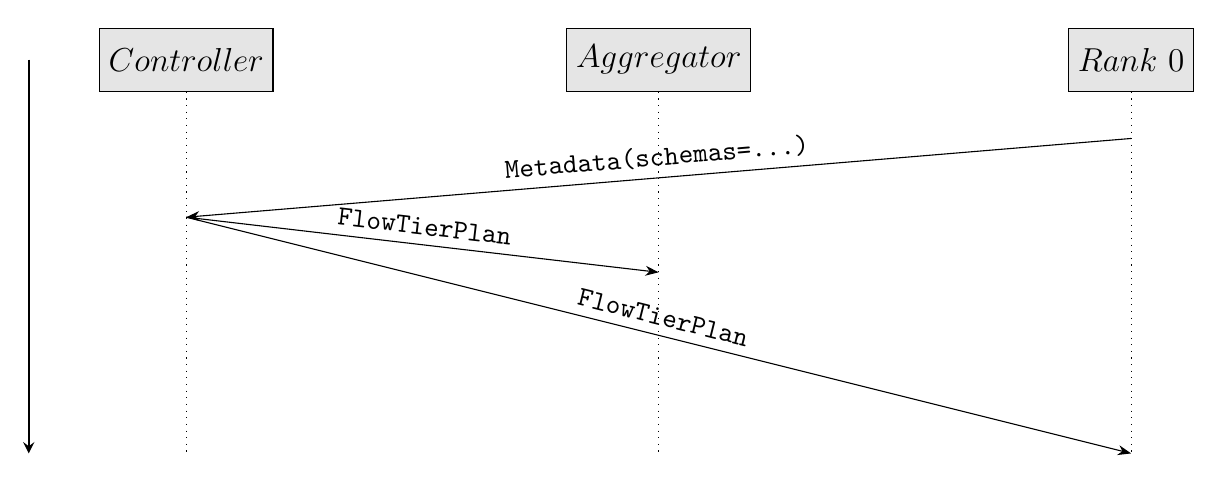
\begin{tikzpicture}[
    rankbox/.style={rectangle, draw, minimum width=1.5cm, minimum height=0.8cm, fill=gray!20, font=\large},
    thread/.style={dotted, thick},
    seqnode/.style={font=\ttfamily\normalsize},
    arrow/.style={->,-Stealth},
    font=\normalsize
  ] % temporary, to visualize grid
  % \draw[step=1cm, gray!10, very thin] (-4, -10) grid (10, 4);
    \rankcontroller{5}

    % flow plan sequence
    % mpi to ctl: Metadata(schemas=...)
    % ctl to agg: FlowPlan([tier0, tier1, ...])
    % ctl to mpi: FlowPlan([tier0, tier1, ...])

    \draw[arrow] ([yshift=-1cm] mpi) -- ([yshift=-2cm] ctl)
        node[midway, above, sloped, seqnode]{Metadata(schemas=...)};
    \draw[arrow] ([yshift=-2cm] ctl) -- ([yshift=-2.7cm] agg)
        node[midway, above, sloped, seqnode]{FlowTierPlan};
    \draw[arrow] ([yshift=-2cm] ctl) -- ([yshift=-5cm] mpi)
        node[midway, above, sloped, seqnode]{FlowTierPlan};
    % 


\end{tikzpicture}
\end{document}

